% \newpage
\section{算法原理}
\subsection{模型基本结构}

本论文采用的图像超分辨率重建的方法,采用了一个被称为Conditional Gated PixelCNN的图像处理模型。我们的模型可以在逻辑上分为两部分,一部分被称为Conditioning network,另一部分为Prior network。

Conditioning network是一个预测模型,其作用是读取低分辩率($16\times16$)图像信息,然后经过批量数据训练,产生尽可能贴合实际的高分辨率还原图像($64\times64$)的输出。Prior network也是一个预测模型,它本质是一个图像生成器。能够按照训练数据的统计特性,生成符合数据规律的图像。在为Prior network提供条件信息的前提下,我们能更高效地指导其生成图像的方向。

Conditioning network的输出能够为Prior network提供条件信息。Prior network根据Conditioning network提供的条件信息,进行调整性的像素预测,生成指定先验知识下的更加合理的图像。所以,本文中两个模型的结合方式是:

\begin{enumerate}
    \item Conditioning network的输出作为Prior network的输入。
    \item Prior network的输出和Conditioning network进行特征图融合作为整体网络输出。
\end{enumerate}

预测过程中,模型的输入为一张$16\times 16$的RGB图像,数据进入到Conditioning network的输入端,Conditioning network能够预测生成一张$64\times 64$的高清晰图像。而后Prior network以Conditioning network的输出作为输入,充分利用其中的条件信息,进行定向性图片生成任务,最终得到一张新的$64\times 64$的图像。在最终输出中,我们将Conditioning network的输出和Prior network的输出做了一个叠加的特征图融合。训练则基于前述的训练过程生成网络输出,利用数据集的标签生成损失值进而进行模型参数训练。

\begin{figure}[htp]
    \centering
    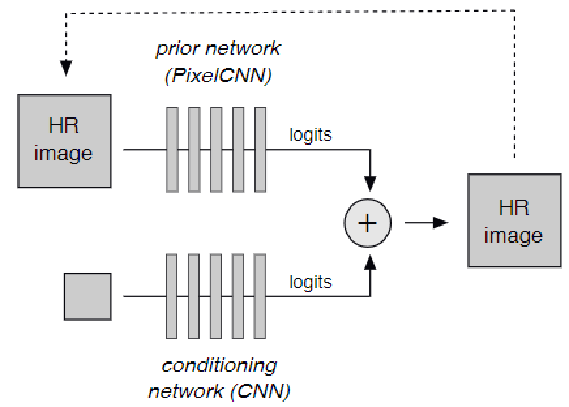
\includegraphics[width=0.4\textwidth]{figures/network}
    \caption{Conditional Gated pixelCNN模型示意图}
\end{figure}

\subsection{Conditioning Network}

根据我们的设计思想,Conditioning network的主要作用是为Prior network提供条件信息,我们所提供的条件信息是和目标预测同分辨率的图片。本论文的实现选用的是反卷积CNN,采用的反卷积CNN网络从一个$16\times 16$的输入开始,分别经过各若干的$1\times 1$卷积层,残差块(Residual Blocks),反卷积层,ReLU(Rectifier Linear Unit)激活层,残差块,$1\times 1$卷积层。

残差块是多层神经网络的堆叠,本文采用的残差块的具体结构是这样的:残差块总体分为5层,残差块第一层为$3\times 3$卷积层,采用same padding,第二层为批量规范化层(Batch Normalization),第三层为ReLU激活层,第四层与第一层的结构相同,第五层与第2层结构相同;整个残差块的输入进入到第一层$3\times 3$卷积层,输出为第五层批量规范化层和网络输入的直接融合;整个网络中,每一层的通道(Channel)数与输入的通道数相同。使用批量规范化层的效果是一方面保持前一层的特征图的数据均值,另一方面减少数据分布的弥散,保持一定的网络训练速度。

\begin{figure}[htp]
    \centering
    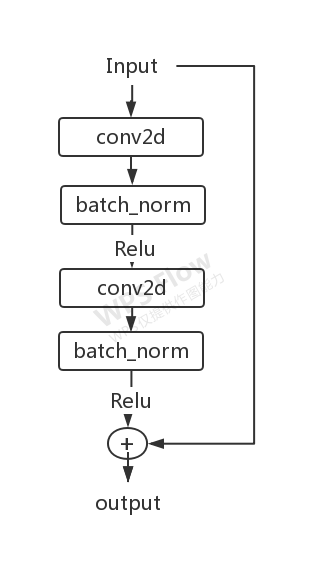
\includegraphics[width=0.2\textwidth]{figures/resnet}
    \caption{残差块结构示意图}
\end{figure}

本文采用的Conditioning network中包含这样一个结构:首先把输入送入$resnum$个残差块,再在残差块后接入一个反卷积层。在数据经过该反卷积层之后,输出特征图的分辨率为输入特征图的2倍。在这之后再接上一个ReLU激活层得到整个残差块的输出。我们将前述的包括残差块到ReLU激活层及其之间各层的多层神经网络堆叠称为一个\textbf{反卷积块(Deconvolution Block)}。

\begin{figure}[htp]
    \centering
    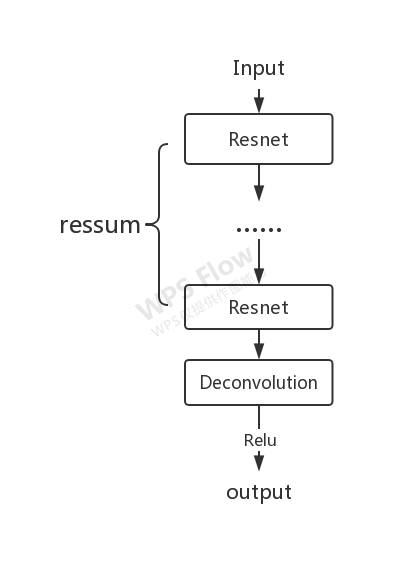
\includegraphics[width=0.3\textwidth]{figures/Deconvolution}
    \caption{反卷积块示意图}
\end{figure}

具体地,我们借助上文所述的几个概念来进一步阐述本论文采用的反卷积CNN的组织结构,其结构图如下所示:

%双栏图片
% \begin{figure*}[htp]
%     \centering
%     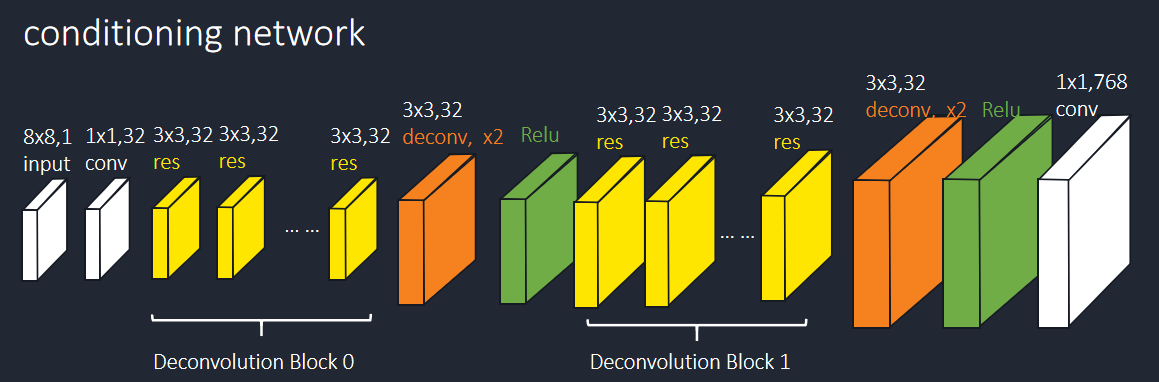
\includegraphics[width=0.8\textwidth]{figures/condition_network}
%     \caption{反卷积CNN结构示意图}
% \end{figure*}
\begin{figure}[htp]
    \centering
    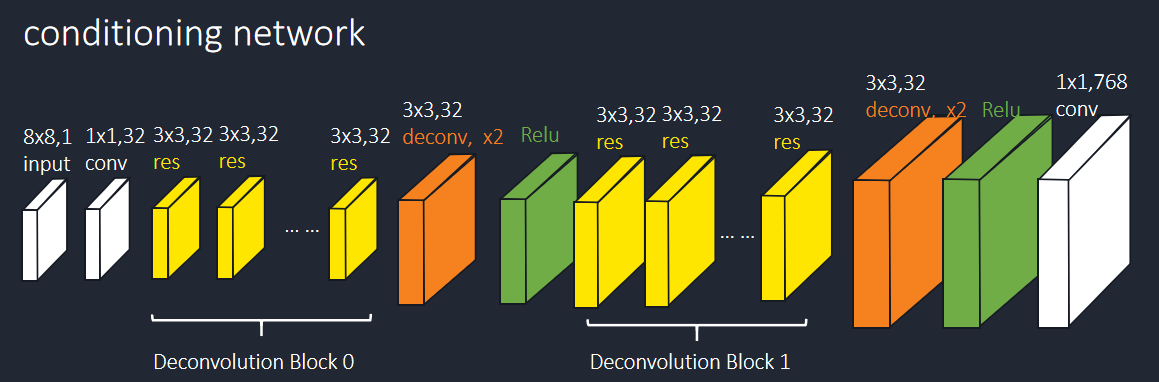
\includegraphics[width=0.5\textwidth]{figures/condition_network}
    \caption{反卷积CNN结构示意图}
\end{figure}

第一层$1\times 1$卷积层的主要作用是将channel数目增加到32个,达到数据升维的效果;而后堆叠两个反卷积块,此时网络大大加深的同时,在输出部分特征图的尺寸已经达到了$64\times 64$,而后接入$resnum$个残差块,最后以一个$1\times 1$卷积层结尾,网络通道数继续增加,达到$768$之多。整个Conditioning network在本实验中展现良好作用的关键点在于模型的:

\begin{enumerate}
    \item 残差块的运用使网络更深,数据内部表征更加丰富,训练效果更好。
    \item 反卷积层的使用,让网络的上采样过程变得可训练,有了更强的分辨率还原能力。
\end{enumerate}

因为Conditioning network和Prior network两者在逻辑上是可分的,因此我们在损失函数方面进行单独考虑,最后使用的是一个混合loss。根据Conditioning network的功能和输出,很自然地,我们希望Conditioning network的输出和标签越接近越好,因此Conditioning network这部分网络的损失函数采用的是数据标签和Conditioning network的输出的softmax loss。

\subsection{Prior network}

Prior network的设计定位是一个条件生成模型,其基本作用是学习如何从Conditioning network产生的条件概率,定向生成最终的图片。本文中的Prior network采用的是一个被称为Gated PixelCNN的模型结构,网络输入和输出都是$32\times 32$的特征图。为逐步阐述清楚Gated PixelCNN的设计思想,我们将逐步介绍Gated PixelCNN的灵感来源和发展。

Gated PixelCNN的灵感来源首先是PixelCNN。PixelCNN是一个像素级图像生成模型,其的结构和CNN尤其是FCN有许多类似之处,最大的区别在于卷积核方面。一个PixelCNN模型可以被很容易地拆分为重复层次的堆叠,其堆叠的一个基本单元我们称为一个\textbf{PixelCNN生成层}。

PixelCNN生成层使用Mask卷积核进行特征图处理,生成层的输入和输出都是一个特征图。Mask卷积核的结构就是在常规卷积核的基础上,增加一个Mask。在PixelCNN当中,有两种Mask,分别为A类Mask和B类Mask,其唯一区别在于,B类Mask的中心元素为1,而A类Mask为0。一个$5\times 5$的A类Mask的结构如图:

\begin{figure}[htp]
    \centering
    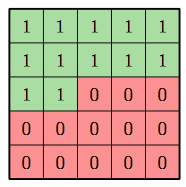
\includegraphics[width=0.3\textwidth]{figures/Mask结构.png}
    \caption{$5\times 5$A类Mask图示}
\end{figure}

在将该Mask与普通卷积核进行逐权重点积之后,再进行常规卷积操作。因为利用了前述的Mask卷积核,PixelCNN在生成当前位置像素的条件概率的时候,仅利用了在卷积核感受野中,处于当前像素位置之前的像素信息,而在当前像素之后的信息则被忽略。PixelCNN模型的算法训练过程中的优化目的是希望对每个标签像素计算到的概率都趋于1,而预测时,我们的Mask卷积核则生成关于颜色的概率密度函数,基于这个函数,我们为新像素填充概率最大的颜色,从而实现图像的生成。

以上就是PixelCNN的基本原理。

PixelCNN的图像生成效率较高,但生成图像素质却不如人意。因为其具有这样的缺点:

\begin{enumerate}
    \item PixelCNN因为受到阶梯状Mask的影响,在多层叠加时产生盲点,其中产生原因见下图
    \item PixelCNN本身建模能力较差
\end{enumerate}

其中盲点是因为PixelCNN在产生所需要的卷积核时,掩盖住了当前像素同一行的右边像素,当多层PixelCNN生成层堆叠时,因为叠加效应使得感受野产生了盲点。

\begin{figure}[htp]
    \centering
    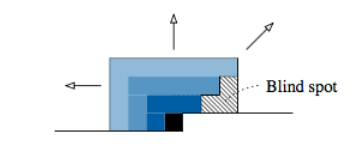
\includegraphics[width=0.3\textwidth]{figures/盲点产生.png}
    \caption{盲点产生图示}
\end{figure}

基于以上的考虑,本文采用了一种改进型的PixelCNN,被称为Gated PixelCNN。Gated PixelCNN为避免盲点问题,采用了改进的Mask卷积核,分为两部分:水平堆(Horizonta Stack)和垂直堆(Vertical Stack),其结构如图7所示。

\begin{figure}[htp]
    \centering
    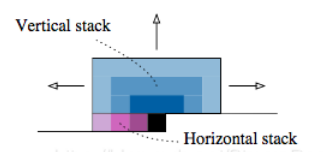
\includegraphics[width=0.3\textwidth]{figures/盲点的消除.png}
    \caption{Gated PixelCNN卷积核图示}
\end{figure}

卷积结果采用两个Mask卷积核的直接相加。因为两个部分的Mask都是矩形,经过堆叠依然是矩形结果,因此Gated PixelCNN就克服了原PixelCNN中产生的盲点问题。

因为需要的网络输出是每个像素的概率信息,因此Prior network采用Loss是Softmax Loss。

\subsection{Conditional Gated PixelCNN}

本论文采用Conditioning network和Prior network按照上文中基本结构进行结合,实现了我们Conditional Gated PixelCNN。PixelCNN本是一种具有随机性的生成模型,在本文中,通过引入Conditional Information,实现了生成模型的生成方向的控制,其中Conditional Information是由Conditioning network提供。

本文中的Conditional Gated PixelCNN的输出是Conditioning network和Prior network的直接叠加。采用的Loss方式是Softmax Loss,其取值等于两个网络模型单独Loss的直接相加。

我们选取这样的Loss以期结合的两个模型都能够得到恰当程度、比例的训练。


